\documentclass[14pt]{article}


\usepackage{etoolbox}
\usepackage[T5]{fontenc}
\usepackage[utf8]{inputenc}
\usepackage[vietnamese,english]{babel}
 \usepackage{array}
 \usepackage{multirow}
 \usepackage{tabu}
 \usepackage{graphicx}
 \usepackage{amsmath}
\usepackage{amsfonts}
\usepackage{amssymb}
\usepackage{blindtext}
\usepackage{quotchap}
\usepackage{dirtytalk}
\usepackage{epigraph}
\usepackage[capposition=top]{floatrow}
\usepackage{biblatex} %Imports biblatex package
\addbibresource{sample.bib} %Import the bibliography file
\usepackage{hyperref}
\hypersetup{
    colorlinks=true,
    linkcolor=blue,
    filecolor=blue,      
    urlcolor=blue,
    pdftitle={Overleaf Example},
    pdfpagemode=FullScreen,
    }
    


\begin{document}

\begin{titlepage}

\newcommand{\HRule}{\rule{\linewidth}{0.5mm}} % Defines a new command for the horizontal lines, change thickness here

\center % Center everything on the page
 
%----------------------------------------------------------------------------------------
%	HEADING SECTIONS
%----------------------------------------------------------------------------------------

\textsc{\LARGE University of Information Technology \\ \\ \\ VNU-HCM }\\[0.5 cm] % Name of your university/college

\textsc{\large Subject: Python for Machine Learning - CS116.M11  }\\[0.5cm] % Minor heading such as course title

%----------------------------------------------------------------------------------------
%	TITLE SECTION
%----------------------------------------------------------------------------------------

\HRule \\[0.4cm]
{ \huge \bfseries Generative Adversarial Networks
}\\[0.4cm] % Title of your document
\HRule \\[0.4cm]
 
%----------------------------------------------------------------------------------------
%	AUTHOR SECTION
%----------------------------------------------------------------------------------------

\begin{minipage}{0.4\textwidth}
\begin{flushleft} \large
\emph{Student: }\\
\textbullet \quad Bùi Khánh Duy\\
ID: 19521418 % Your name
\end{flushleft}
\end{minipage}
~
\begin{minipage}{0.4\textwidth}
\begin{flushright} \large
\emph{Lecturer:} \\
Nguyễn Vĩnh Tiệp % Supervisor's Name
\end{flushright}
\end{minipage}\\[2cm]

% If you don't want a supervisor, uncomment the two lines below and remove the section above
%\Large \emph{Author:}\\
%John \textsc{Smith}\\[3cm] % Your name

%----------------------------------------------------------------------------------------
%	DATE SECTION
%----------------------------------------------------------------------------------------

% I don't want day because it is English
% {\large \today}\\[2cm] % Date, change the \today to a set date if you want to be precise

%----------------------------------------------------------------------------------------
%	LOGO SECTION
%----------------------------------------------------------------------------------------


\includegraphics{logo-uit.png}\\ % Include a department/university logo - this will require the graphicx package
 
%----------------------------------------------------------------------------------------

\vfill % Fill the rest of the page with whitespace

\end{titlepage}

\newpage
\tableofcontents
\section{About GANs}
\\
\epigraph{Generative Adversarial Networks is the most interesting idea in the last 10 years in Machine Learning.}{\textit{ Yann LeCun \\ Director of AI Research at Facebook AI}}
\\
A generative adversarial network is a class of machine learning frameworks  based on generative model that’s use for unsupervised learning. 
\\
It has two neural networks compete with each other to become more accurate in their predictions. 
\begin{center}
    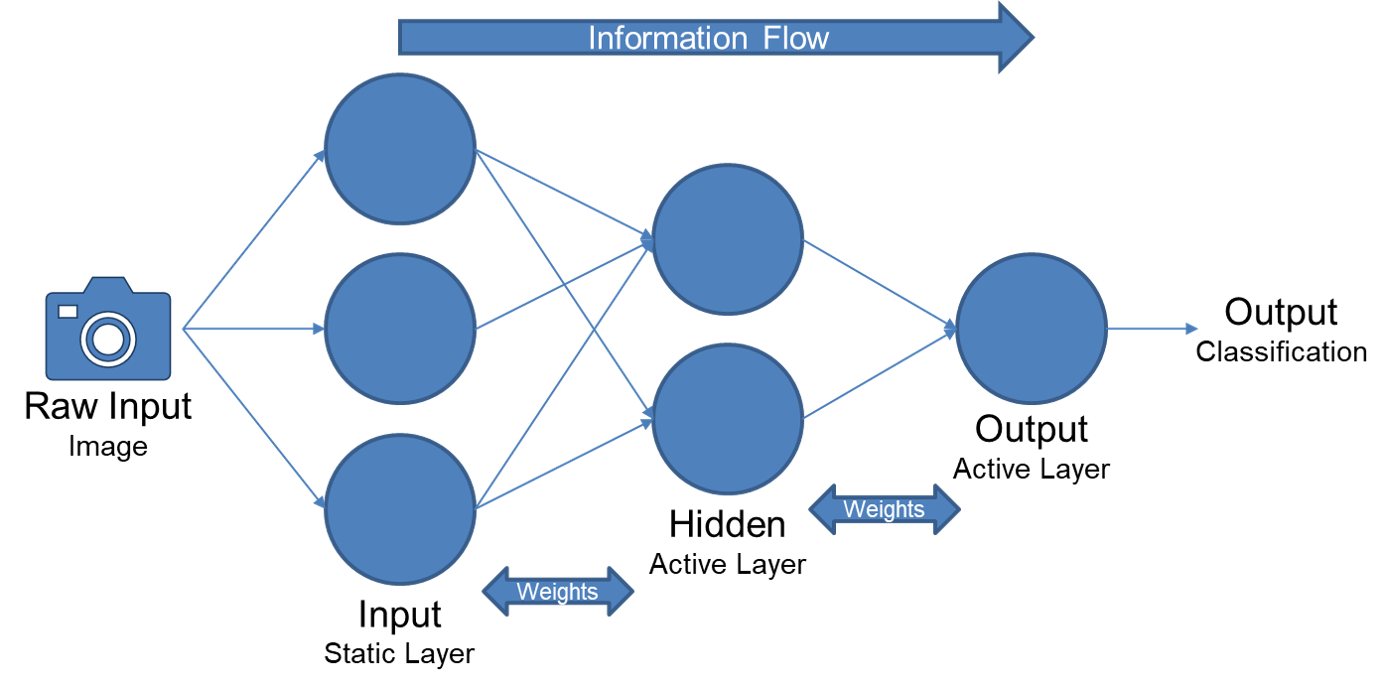
\includegraphics[width = 11 cm ]{1.png}
\end{center}
\\
The two neural networks that make up a GAN are referred to as the generator and the discriminator.
\\ \\ 
\hspace*{1cm} \textit{"Generative adversarial networks are based on a game theoretic scenario in which the generator network must compete against an adversary. The generator network directly produces samples. Its adversary, the discriminator network, attempts to distinguish between samples drawn from the training data and samples drawn from the generator."}\\
\hspace*{5cm} -- Page 699, \href{https://www.amazon.com/Deep-Learning-Adaptive-Computation-Machine/dp/0262035618/ref=as_li_ss_tl?keywords=deep+learning&qid=1553730173&s=books&sr=1-1&linkCode=sl1&tag=inspiredalgor-20&linkId=e9ef92a6248b927689728a8bf72b7cd1&language=en_US}{Deep Learning}, 2016.--  
\\
The generator is a convolutional neural network and the discriminator is a deconvolutional neural network. The aim of the generator is to artificially manufacture outputs that could easily be mistaken for real data. The aim of the discriminator is to identify which outputs it receives have been artificially created. 
\\ 
Essentially, GANs create their very own training data. as the feedback loop among the adversarial networks continues, the generator will begin to produce higher-quality output and the discriminator becomes better at flagging data that has been artificially created. 
generative adversarial networks (GANs) have grow to be a research focus of artificial intelligence. stimulated by means of -player zero-sum game, GANs include a generator and a discriminator, both trained under the adversarial learning idea. 
\\
The purpose of GANs is to estimate the potential distribution of real data samples and generate new samples from that distribution. since their initiation, GANs had been broadly studied due to their sizeable prospect for programs, together with image and vision computing, speech and language processing, and so forth.  simply, GANs can offer great algorithmic help for parallel intelligence. 
\\ 
\section{How does a GANs work?}
\\
Originally conceived within the early 1940s as a mathematical construct, the artificial neural network was popularized within the 1980s through a technique called backpropagation. Backprop, for short, allows a synthetic neural network to regulate the weights of every layer at every epoch of coaching. within the 1980s, the boundaries of computational power only allowed for a specific level of coaching. because the computing power expanded and therefore the research grew, there was a renaissance with Machine Learning.
\\
With the appearance of cheap computing power, a replacement technique was born: deep neural networks. Utilizing the flexibility of GPUs to compute tensors very quickly, some libraries are developed to make these deep neural networks. To become a deep neural network, the fundamental premise is this: add four or more hidden layers between the input and output. Typically, there are thousands of neurons within the graph and also the neural network features a much larger capacity to find out. This construct is illustrated within the following diagram.
\\
\begin{center}
    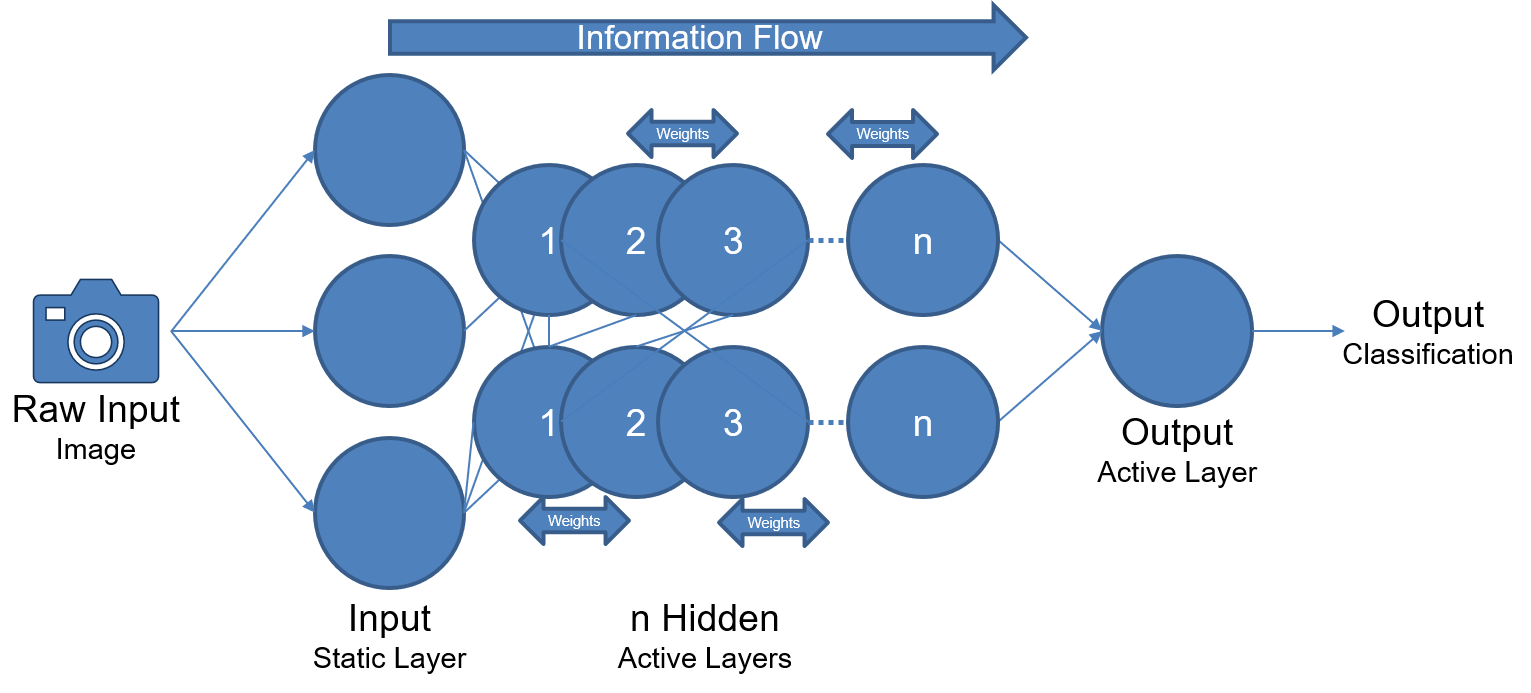
\includegraphics[width = 11 cm ]{2.png}
\end{center}
\\
A deep neural network is a relatively straightforward expansion of the neural network's basic architecture.
\\
This diagram depicts the fundamental structure of a deep neural network. This architecture can be modified and restructured in many ways, but this basic graph has all of the necessary components to build a Deep Neural Network.
\\
\begin{center}
    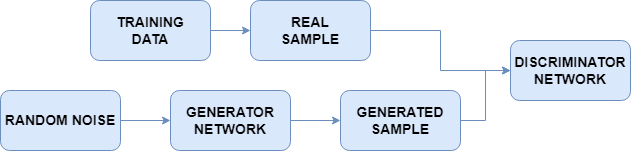
\includegraphics[width = 11 cm ]{3.png}
\end{center}
\\
Identifying the intended end product and gathering an initial training dataset based on those parameters is the first step in constructing a GAN. This data is then randomized and put into the generator until it reaches a baseline level of output accuracy.
\\
The generated graphics, together with real data points from the original concept, are sent into the discriminator after that. The discriminator sorts through the data and assigns each picture an authenticity probability between 0 and 1. (1 correlates with real and 0 correlates with fake).
\\
\begin{center}
    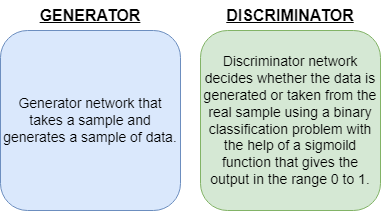
\includegraphics[width = 11 cm ]{4.png}
\end{center}
\\
These values are manually verified for success, and the process is repeated until the desired result is achieved.
\\
\section{Training GANs }
\\
\subsection{Train the discriminator}
\\
\begin{center}
    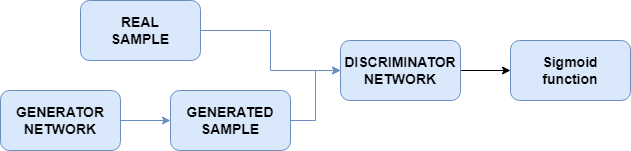
\includegraphics[width = 11 cm ]{5.png}
\end{center}
\\
Train the discriminator and freeze the generator, which means the generator's training set is set to false and the network will only do forward passes with no back-propagation.\\
Actually, it just means that the discriminator is trained with real data and tested to see if it can properly predict them, and then tested again with fake data to see if it can recognize them as fake.
\\
\subsection{Train the generator}
\\

\\
\begin{center}
    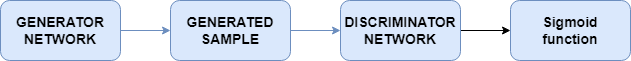
\includegraphics[width = 11 cm ]{6.png}
\end{center}
\\
Train the generator and freeze the discriminator in the same way that you trained the discriminator. In this step, we take the results from the previous phase and utilize them to improve the prior state in order to mislead the discriminator more effectively.
\\
\subsection{Step-by-step}
\\
\\\textbf{Step 1:} Define the problem
\\
\textbf{Step 2:} Choose architecture of GANs
\\\textbf{Step 3:} Train discriminator on real data
\\\textbf{Step 4:} Generate fake inputs for generator
\\\textbf{Step 5:} Train discriminator on fake data
\\ \textbf{Step 6:} Train the generator with the output of discriminator
\\
\section{Loss function}
The standard GAN loss function, also known as the min-max loss, was first described in a 2014 paper by Ian Goodfellow et al., titled \href{https://arxiv.org/abs/1406.2661}{“Generative Adversarial Networks“}.
\\
\begin{center}
    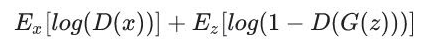
\includegraphics[width = 11 cm ]{7.png}
\end{center}
\\
In this function:\\
\hspace*{0.3cm} $D_(_x_)$ is the discriminator's estimate of the probability that real data instance x is real.
\\
\hspace*{0.3cm} $E_x$ is the expected value over all real data instances.\\
\hspace*{0.3cm} $G_(_z_)$ is the generator's output when given noise z.\\
\hspace*{0.3cm} $D(G_(_z_))$ is the discriminator's estimate of the probability that a fake instance is real.\\
\hspace*{0.3cm} $E_z$ is the expected value over all random inputs to the generator (in effect, the expected value over all generated fake instances $G_(_z_)$.\\
The formula derives from the \href{https://developers.google.com/machine-learning/glossary#cross-entropy
}{cross-entropy} between the real and generated distributions.
\\The generator can't directly affect the $log(D(x))$ term in the function, so, for the generator, minimizing the loss is equivalent to minimizing $log(1 - D(G_(_z_)))$
\\
This function is minimized by the generator, whereas it is maximized by the discriminator. This description of the loss seems effective when seen as a min-max game. In actuality, it saturates for the generator, which means that if it doesn't catch up with the discriminator, the generator will frequently cease training.
\\
\textbf{The Discriminator loss} and \textbf{Generator loss sections} of the Standard GAN loss function can be further divided.
\\
\subsection{Generator loss}
\\
\begin{center}
    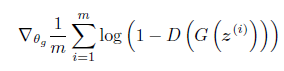
\includegraphics[width = 11 cm ]{8.png}
\end{center}
\\
\subsection{Discriminator loss }

\\
\begin{center}
    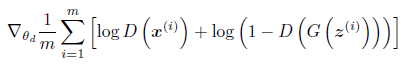
\includegraphics[width = 11 cm ]{9.png}
\end{center}
\\
\begin{center}
    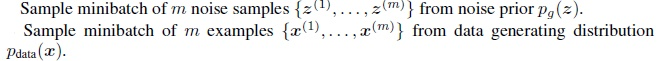
\includegraphics[width = 12 cm ]{10.jpg}
\end{center}
\section{Make Trainings GANs more stable}
\\
It's tough to train GANs.\\
Because both the generator and discriminator models are trained concurrently in a game, they are challenging to train. As a result, advancements to one model come at the price of the other.
\\
\hspace*{1cm} \textit{“Training GANs consists in finding a Nash equilibrium to a two-player non-cooperative game. […] Unfortunately, finding Nash equilibria is a very difficult problem. Algorithms exist for specialized cases, but we are not aware of any that are feasible to apply to the GAN game, where the cost functions are non-convex, the parameters are continuous, and the parameter space is extremely high-dimensional"}
\hspace*{4cm} -- \hyperlink{https://arxiv.org/abs/1606.03498}{Improved Techniques for Training GANs}, 2016 -- 
\\
As a result, we'll have a means to make GAN training more stable.
\\
\subsection{Use Strided Convolutions}
\\
Pooling layers, such as max-pooling layers, are commonly used in convolutional neural networks for downsampling.\\
Instead of using pooling layers in GANs, stride in convolutional layers should be used to achieve downsampling in the discriminator model.For upsampling, fractional stride (deconvolutional layers) can also be utilized in the generator.
\\
\begin{center}
    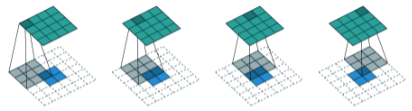
\includegraphics[width = 12 cm ]{16.png}
\end{center}
\\ \\
\hspace*{1cm} \textit{Deterministic spatial pooling functions (such as max pooling) with strided convolutions, allowing the network to learn its own spatial downsampling. We use this approach in our generator, allowing it to learn its own spatial upsampling, and discriminator.}
\\

\hspace*{4cm} --
\hyperlink{https://arxiv.org/abs/1511.06434}{Unsupervised Representation Learning with Deep Convolutional Generative Adversarial Networks} ,2015
\\
\subsection{Remove Fully-Connected Layers}
\\
Fully-connected layers are commonly used following feature extraction layers in convolutional layers as an interpretation of the retrieved features prior to the model's output layers.\\
Fully-connected layers aren't employed in GANs, and the discriminator and convolutional layers are flattened and transmitted directly to the output layer.
In addition, the random Gaussian input vector provided to the generator model is immediately transformed into a multi-dimensional tensor that can be sent to the first convolutional layer and upscaled.\\ 
\begin{center}
    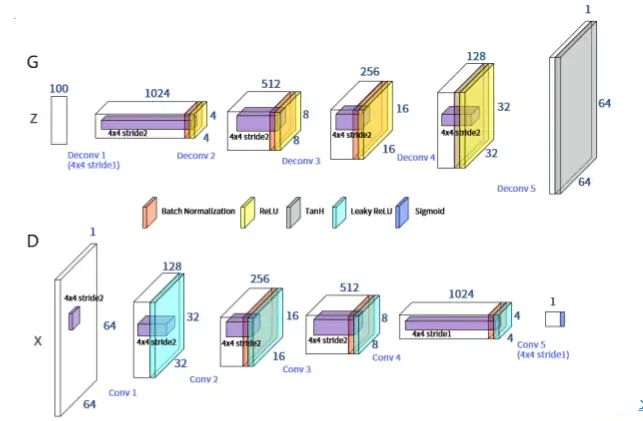
\includegraphics[width = 12 cm ]{fully.png}
\end{center} \\ \\
\hspace*{1cm} \textit{The first layer of the GAN, which takes a uniform noise distribution Z as input, could be called fully connected as it is just a matrix multiplication, but the result is reshaped into a 4-dimensional tensor and used as the start of the convolution stack. For the discriminator, the last convolution layer is flattened and then fed into a single sigmoid output.}
\\
\hspace*{4cm} --
\hyperlink{https://arxiv.org/abs/1511.06434}{Unsupervised Representation Learning with Deep Convolutional Generative Adversarial Networks} ,2015
\\
\subsection{Use Batch Normalization}
\\
\hyperlink{https://machinelearningmastery.com/how-to-accelerate-learning-of-deep-neural-networks-with-batch-normalization/}{Batch normalization} standardizes the activations from a prior layer to have a zero mean and unit variance. \\
When training deep convolutional neural networks, batch normalization has become standard practice, and GANs are no exception. Except for the output of the generator and the input to the discriminator, batch norm layers are suggested in both the discriminator and generator models.
\\ 
\begin{center}
    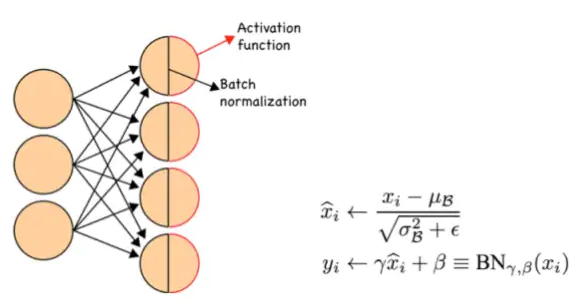
\includegraphics[width = 12 cm ]{batch.png}
\end{center} \\ \\ 
\hspace*{1cm} \textit{Directly applying batchnorm to all layers however, resulted in sample oscillation and model instability. This was avoided by not applying batchnorm to the generator output layer and the discriminator input layer.}\\
\hspace*{4cm} --
\hyperlink{https://arxiv.org/abs/1511.06434}{Unsupervised Representation Learning with Deep Convolutional Generative Adversarial Networks} ,2015
\\
\subsection{Use ReLU, Leaky ReLU, and Tanh}
In deep convolutional neural networks, activation functions like \hyperlink{https://machinelearningmastery.com/how-to-fix-vanishing-gradients-using-the-rectified-linear-activation-function/}{ReLU} are utilized to overcome the vanishing gradient problem and favor sparse activations (e.g. lots of zero values).\\
For the generator model, ReLU is suggested, but not for the discriminator model. Instead, in the discriminator, Leaky ReLU, a variant of ReLU that accepts values smaller than zero, is selected.
\\ 
\begin{center}
    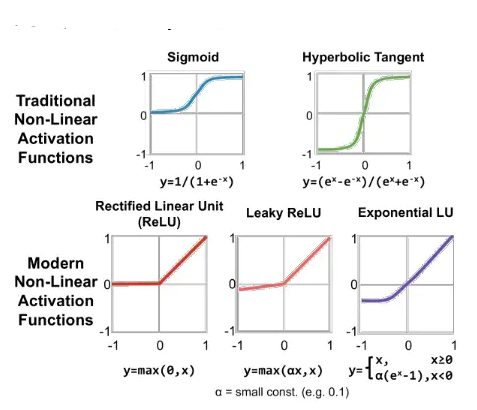
\includegraphics[width = 7 cm ]{relu.png}
    \\ \\ 
\end{center} 
\hspace*{1cm} \textit{The ReLU activation is used in the generator with the exception of the output layer which uses the Tanh function. […] Within the discriminator we found the leaky rectified activation to work well …}
\\
\hspace*{4cm} --
\hyperlink{https://arxiv.org/abs/1511.06434}{Unsupervised Representation Learning with Deep Convolutional Generative Adversarial Networks} ,2015
\\
In addition, the generator's output layer employs the hyperbolic tangent (tanh) activation function, and the generator's and discriminator's inputs are scaled to the range [-1, 1].\\
The slope of the Leaky ReLU in the discriminator was set to 0.2, and the model weights were set to tiny \hyperlink{https://machinelearningmastery.com/how-to-generate-random-numbers-in-python/}{Gaussian random values}.\\
\subsection{Use Adam Optimization}
\\ 
With a batch size of 128 pictures, both the generator and discriminator are trained using stochastic gradient descent.
\\ \\ 
\hspace*{1cm} \textit{All models were trained with mini-batch stochastic gradient descent (SGD) with a mini-batch size of 128}\\ 
\hspace*{4cm} --
\hyperlink{https://arxiv.org/abs/1511.06434}{Unsupervised Representation Learning with Deep Convolutional Generative Adversarial Networks} ,2015
\\ \\
The models were trained using the \hyperlink{https://machinelearningmastery.com/adam-optimization-algorithm-for-deep-learning/}{Adam version of stochastic gradient descent} with a learning rate of 0.0002 and a momentum (beta1) of 0.5.
\\ \\ 
\hspace*{1cm} \textit{We used the Adam optimizer with tuned hyperparameters. We found the suggested learning rate of 0.001, to be too high, using 0.0002 instead. Additionally, we found leaving the momentum term β1 at the suggested value of 0.9 resulted in training oscillation and instability while reducing it to 0.5 helped stabilize training.}\\ 
\hspace*{4cm} --
\hyperlink{https://arxiv.org/abs/1511.06434}{Unsupervised Representation Learning with Deep Convolutional Generative Adversarial Networks} ,2015
\\ 
\section{Advantages and disadvantages of GANs }\\
\subsection{Advantages}
1. GANs generate data that resembles the original data. When you feed GAN an image, it will create a new version of the image that is similar to the original. It can also produce alternative versions of text, video, and audio.


\begin{center}
    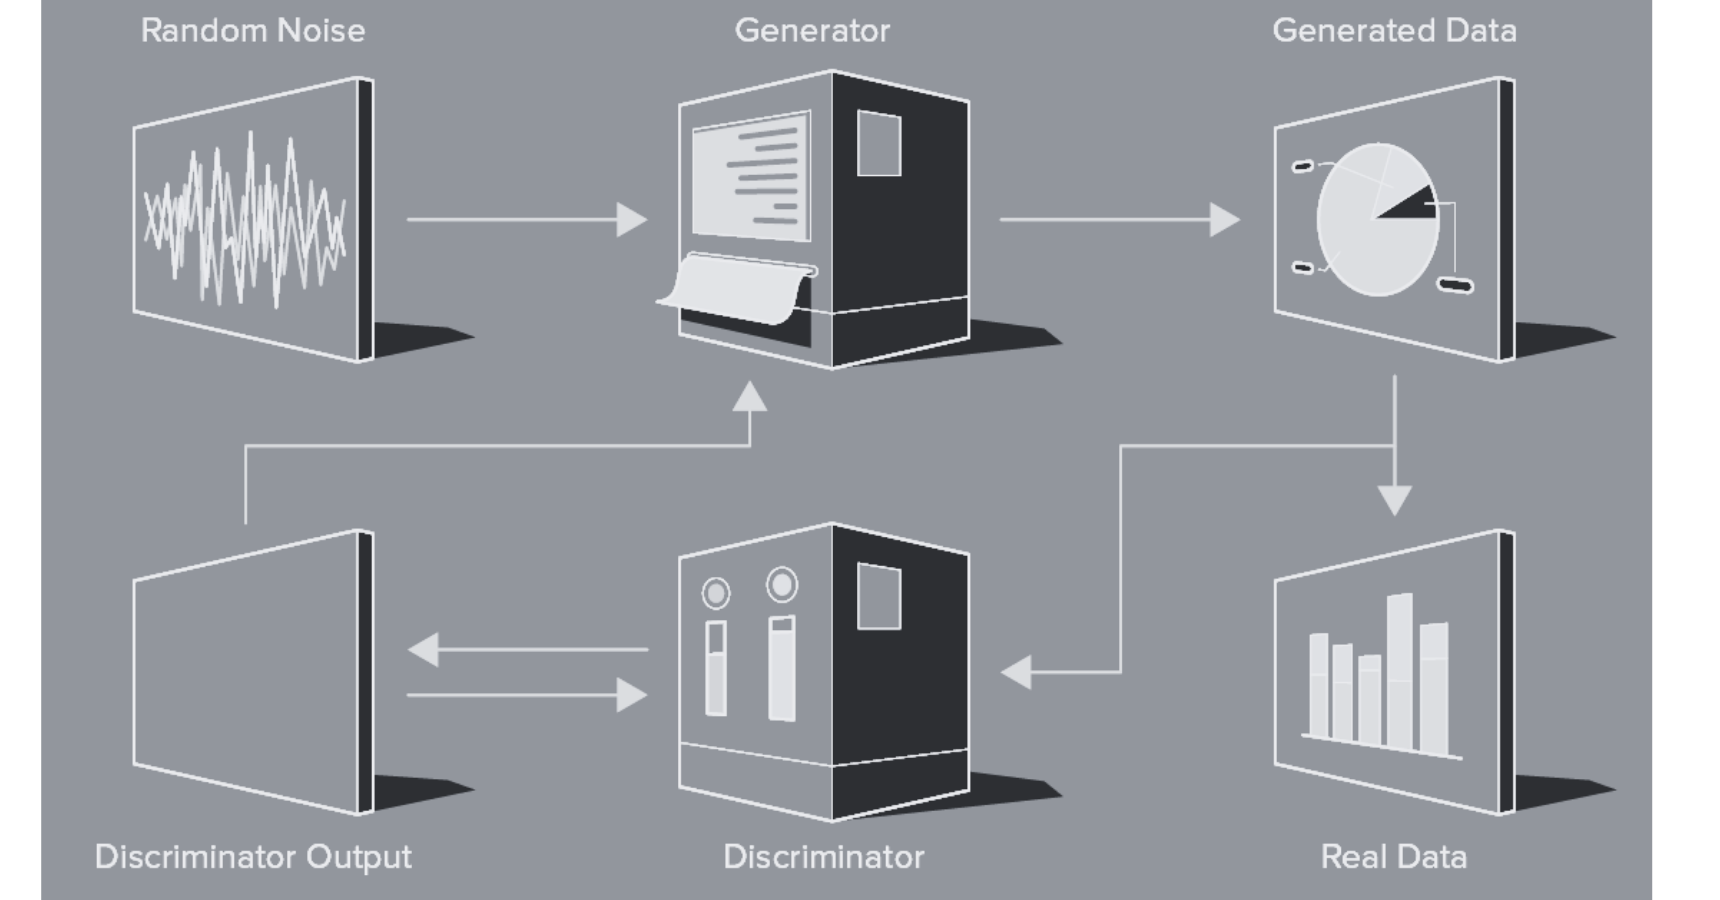
\includegraphics[width = 12 cm ]{20.png}
    \\ \\ 
\end{center} 
2. GANs delve into the details of data and can readily translate them into multiple forms, making them useful in machine learning.
\\
3. We can readily recognize trees, streets, bicyclists, people, and parked automobiles using GANs and machine learning, and we can also measure the distance between different objects.
\\
\subsection{Disadvantages}
\\
1. More difficult to train: It require continually submit new sorts of data to see if it performs correctly.
\\
2. Generating outcomes from text or speech is a difficult task.
\\
3. "Realistic," but not real. Fake patterns can be made, particularly for tiny size structures or non-natural objects such as text -> loss function issue.
\\


\section{Testing and evalution}\\
\subsection{Auto generate images}\\
\textbf{DATASET}\\
We'll utilize the Cats Faces Dataset, which contains around 15,700 photos of cats. There are no labels on the photos since generative modeling is an unsupervised learning approach. The dataset has a single folder called cats, which contains almost 15,700 JPG photos.
\\
\begin{center}
    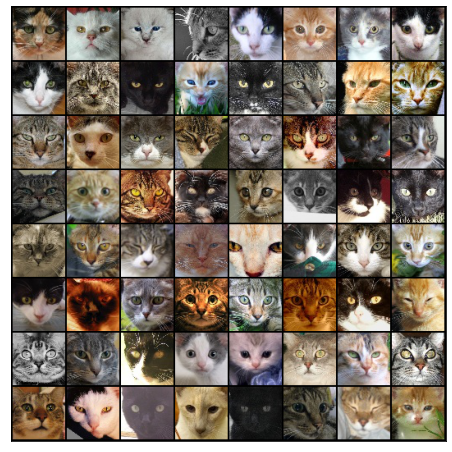
\includegraphics[width = 9 cm ]{dataset_cat.png}
    \\ \\ 
\end{center} 
\\
After training the model for 60 epochs we can see the generated images. 
\\
\begin{center}
    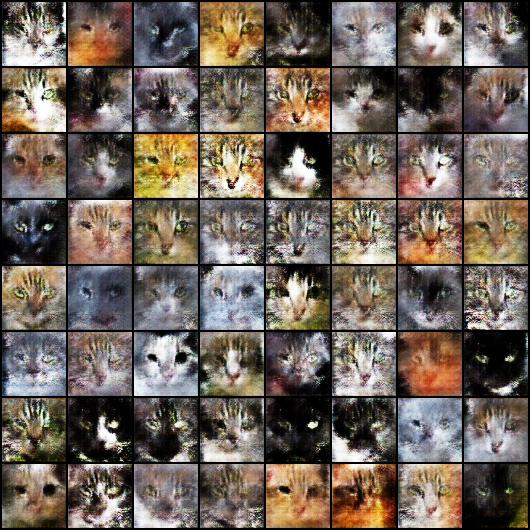
\includegraphics[width = 8.5 cm ]{25.png}
    \\ \\ 
\end{center} 
As we can see the generated images from the model are similar to real ones. 
\\
Plot of Losses of the Model
\\
\begin{center}
    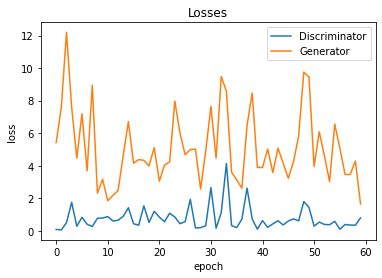
\includegraphics[width = 7 cm ]{26.png}
    \\ \\ 
\end{center}
Plot of Scores of the Model
\\
\begin{center}
    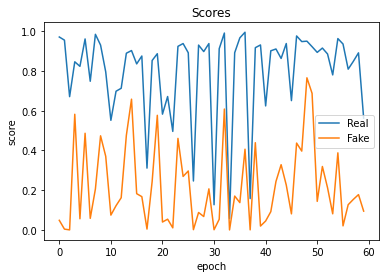
\includegraphics[width = 7 cm ]{27.png}
    \\ \\ 
\end{center}
\subsection{Image colorization}
\\
In this example, we’ll use GAN to colorize a grayscale (black/white) image.\\
\\
\textbf{DATASET}
\\
A dataset of RGB images to train the GAN model more than 2500 images whose images consists of various scenes/places.  Since generative modeling is an unsupervised learning method, hence there are no labels on the images. The dataset has a single folder named data which contains more than 2500+ images in JPG format.
\\

\begin{center}
    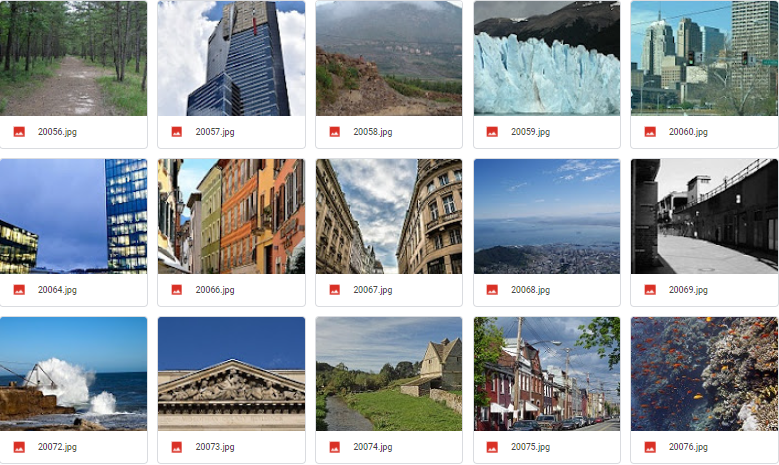
\includegraphics[width = 12 cm ]{23.png}
    \\ \\ 
\end{center} 
After training the model for 150 epochs we can see the generated images. There are 2 example: \\
\begin{center}
    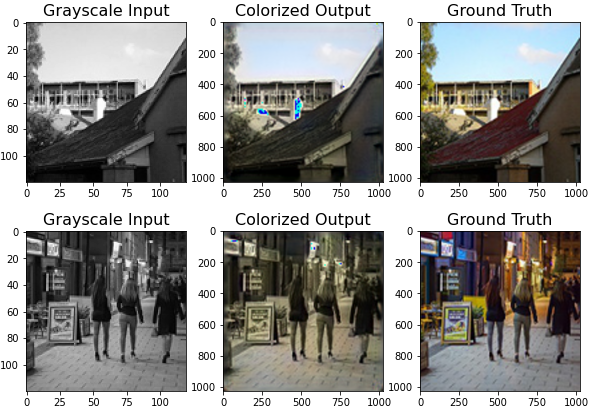
\includegraphics[width = 12 cm ]{24.png}
    \\ \\ 
\end{center} 



\\
\section{GANs application}
\subsection{Image to image translator}
Phillip Isola, et al. in their 2016 paper titled “\hyperlink{https://arxiv.org/abs/1611.07004}{Image-to-Image Translation with Conditional Adversarial Networks}” demonstrate GANs, specifically their pix2pix approach for many image-to-image translation tasks.
\\
Examples include translation tasks such as:\\
\hspace*{1cm}Translation of semantic images to photographs of cityscapes and buildings.
\\
\hspace*{1cm}Translation of satellite photographs to Google Maps.
\\
\hspace*{1cm}Translation of photos from day to night.\\
\hspace*{1cm}Translation of black and white photographs to color.\\
\hspace*{1cm}Translation of sketches to color photographs.\\

\begin{center}
    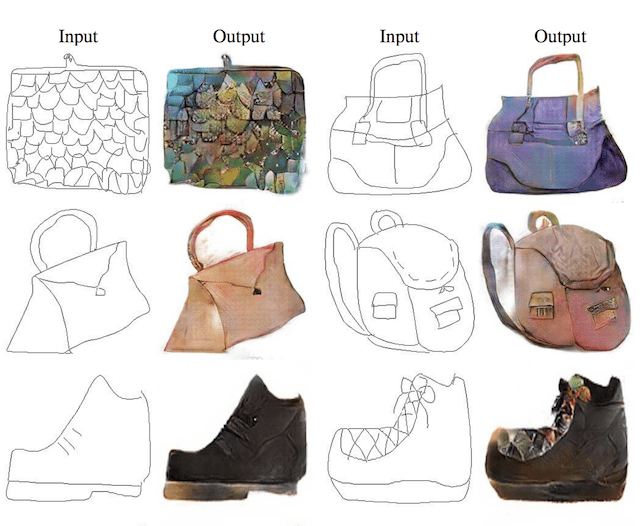
\includegraphics[width = 11 cm ]{11.png}
    Example of Sketches to Color Photographs With pix2pix.Taken from Image-to-Image Translation with Conditional Adversarial Networks, 2016.
\end{center}
\\
Jun-Yan Zhu in their 2017 paper titled “\hyperlink{https://arxiv.org/abs/1703.10593}{Unpaired Image-to-Image Translation using Cycle-Consistent Adversarial Networks}” introduce their famous \hyperlink{https://junyanz.github.io/CycleGAN/}{CycleGAN} and a suite of very impressive image-to-image translation examples.\\
\\
\\
\\
The example below demonstrates four image translation cases:\\
\hspace*{1cm}Translation of semantic images to photographs of cityscapes and buildings.
\\
\hspace*{1cm}Translation from photograph to artistic painting style.
\\
\hspace*{1cm}Translation of horse to zebra.\\
\hspace*{1cm}Translation of photograph from summer to winter.\\
\hspace*{1cm}Translation of satellite photograph to Google Maps view.\\

\begin{center}
    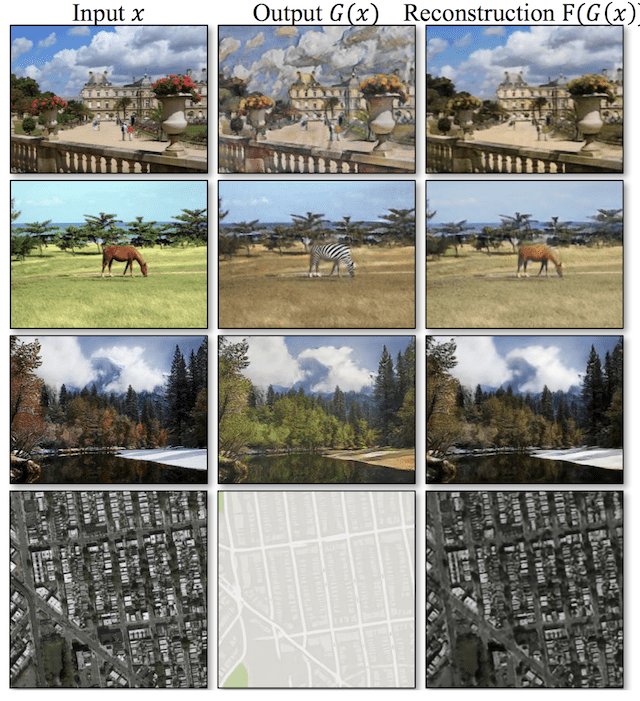
\includegraphics[width = 11 cm ]{12.png}
    Example of Four Image-to-Image Translations Performed With CycleGANTaken from Unpaired Image-to-Image Translation using Cycle-Consistent Adversarial Networks, 2017.
\end{center}
\\
The paper also provides many other examples, such as:\\
\hspace*{1cm}Translation of painting to photograph.
\\
\hspace*{1cm}Translation of sketch to photograph.
\\
\hspace*{1cm}Translation of apples to oranges.\\
\hspace*{1cm}Translation of photograph to artistic painting.\\

\begin{center}
    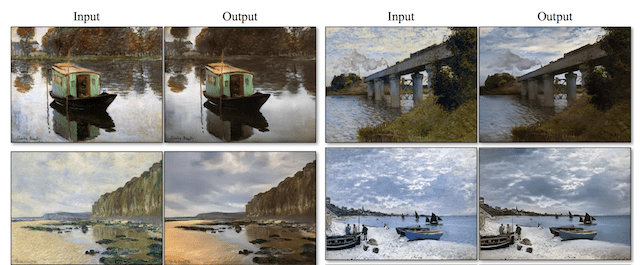
\includegraphics[width = 11 cm ]{13.png}
    Example of Translation from Paintings to Photographs With CycleGAN.Taken from Unpaired Image-to-Image Translation using Cycle-Consistent Adversarial Networks, 2017.
\end{center}

\\
\subsection{Generating a realistic image from text (text2image)}
\\
Han Zhang, et al. in their 2016 paper titled “\hyperlink{https://arxiv.org/abs/1612.03242}{StackGAN: Text to Photo-realistic Image Synthesis with Stacked Generative Adversarial Networks}” demonstrate the use of GANs, specifically their StackGAN to generate realistic looking photographs from textual descriptions of simple objects like birds and flowers.
\\
\begin{center}
    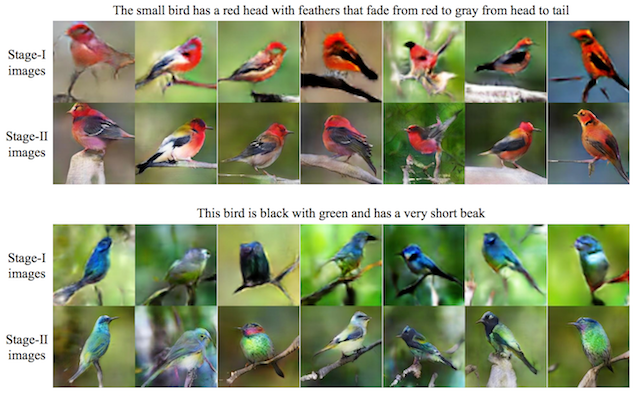
\includegraphics[width = 11 cm ]{14.png}
    Example of Textual Descriptions and GAN-Generated Photographs of BirdsTaken from StackGAN: Text to Photo-realistic Image Synthesis with Stacked Generative Adversarial Networks, 2016.
\end{center}
\\
\subsection{Predict subsequent video frames}
\\
Carl Vondrick, et al. in their 2016 paper titled “\hyperlink{https://arxiv.org/abs/1609.02612}{Generating Videos with Scene Dynamics}” describe the use of GANs for video prediction. Specifically, successfully predicting up to a second of video frames, mostly for static scene features.
\\

\begin{center}
    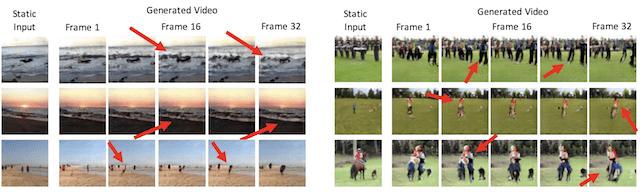
\includegraphics[width = 11 cm ]{15.png}
    Example of Video Frames Generated With a GAN.Taken from Generating Videos with Scene Dynamics, 2016.
\end{center}
\\
Besides, GANs also can filling in images from an outline, converting black and white imagery into color,etc...
\\
\section{The difference between GANs and others}

\subsection{Gans generator and VAE's encoder}
\\
\textbf{A GANs generator} generates a picture by sampling from a low-dimensional random variable. The discriminator then examines the image and determines whether it corresponds to a target distribution or not. We may produce an expansion of pictures simply by sampling the preliminary random variable and sending via the generator once it has been trained.\\
\textbf{The encoder of a VAE} compresses an image from a goal distribution into a low-dimensional latent space. The decoder's job then is to use that latent space representation to recreate the original image. We can generate latent space representations of numerous images and interpolate among them once the network has been trained, before forwarding via the decoder, which generates new images.
\\
GANs usually produce better photo-realistic pictures however can be tough to work with. Conversely, VAEs are simpler to train however don’t normally provide the quality results.
\\
\subsection{GANs and CNN}
\\
GAN is a better classifier and data synthehsizer than CNN; it can function with less data, but CNN requires a lot of data. Furthermore, GANs state of the art models. GANs are useful for segmentation and classification, while CNNs are the most accurate (If dataset is large)
\\
\section{The development trends of GANs}
\\
How to produce a range of data that can interact with people from basic random inputs is an essential research path in the near future from the standpoint of building and implementing GANs. How to combine GANs with feature learning, imitation learning, and reinforcement learning to build new AI applications and support the development of these techniques is highly important from the standpoint of merging GANs and other methods. In the long term, how to employ GANs to encourage AI development and application, improve AI's capacity to perceive the environment, and even inspire AI creativity are crucial issues that academics should examine.
\\
\section{Conclusion}
\\

The development of generative models relies heavily on GANs. GANs solve the problem of generating data that can be naturally interpreted as a powerful class of generative methods. The selected neural network topology does not limit the generation dimension, which substantially broadens the scope of the generated data samples, especially for the development of high-dimensional data. Furthermore, the neural network topology may incorporate a variety of loss functions, giving the model designer more flexibility. GANs are trained using two adversarial neural networks as a training criterion and can be trained using backpropagation in general. GANs' generation process does not necessitate a time-consuming sampling sequence; instead, they can directly sample and predict new samples, increasing the efficiency of generating new samples. In summary, GANs offer a potential method for creating data that is relevant to people.GANs have not only contributed significantly to the development of generative models, but they are also useful and instructive for semi-supervised learning.

\section{References}
\\
[1] Nguyen Canh, Thuong. (2018). Re: Can anyone inform me please about the advantages and limitations of Generative Adversarial Networks (GANs) ?.\\
Retrieved from:\\ \url{https://www.researchgate.net/post/Can-anyone-inform-me-please-about-the-advantages-and-limitations-of-Generative-Adversarial-Networks-GANs/5b36e1ca6a21fff96939d7cf/citation/download.} 
\\ \\ 
[2] Alexander Soare, (2021), Re: What are the fundamental differences between VAE and GAN for image generation? \\
Retrieved from: \\
\url{https://ai.stackexchange.com/questions/25601/what-are-the-fundamental-differences-between-vae-and-gan-for-image-generation}
\\
\\
[3] Nathan Yan (2020) Re: \url{https://www.quora.com/Whats-the-difference-between-CNN-GANs-autoencoders-and-VAE}\\  Retrieved from: 
\\

What's the difference between CNN, GANs, autoencoders and VAE? - Quora 
\\
\\
[4] Image Colorization Using GANs | Deep Learning | TensorFlow | Python, by Efshal Ahmed Muhammad Hassan, Coderz Den 
\\
\\
[5] Loss function from Google Developer website.\\ Retrieved from:\\ \url{https://developers.google.com/machine-learning/gan/loss }
\\ \\ 
[6] Phillip Isola, Jun-Yan Zhu, Tinghui Zhou, Alexei A. Efros, 2016, Image-to-Image Translation with Conditional Adversarial Networks, Computer Vision and Pattern Recognition (cs.CV), pp. 12.
\\\url{https://arxiv.org/abs/1611.07004} [cs.CV] 
\\
\\
[7] Jun-Yan Zhu, Taesung Park, Phillip Isola, Alexei A. Efros. 2017, Unpaired Image-to-Image Translation using Cycle-Consistent Adversarial Networks, Computer Vision and Pattern Recognition (cs.CV),  pp. 3-11 
\\
\url{https://arxiv.org/abs/1611.07004} [cs.CV] 
\\
\\
[8] Han Zhang, Tao Xu, Hongsheng Li, Shaoting Zhang, Xiaogang Wang, Xiaolei Huang, Dimitris Metaxas, 2016, StackGAN: Text to Photo-realistic Image Synthesis with Stacked Generative Adversarial Networks, Computer Vision and Pattern Recognition (cs.CV); Artificial Intelligence (cs.AI); Machine Learning (stat.ML), pp. 11.\\
\url{https://arxiv.org/abs/1612.03242} [cs.CV] 
\\
\\
[9] Carl Vondrick, Hamed Pirsiavash, Antonio Torralba, 2016, Generating Videos with Scene Dynamics, Computer Vision and Pattern Recognition (cs.CV); Graphics (cs.GR); Machine Learning (cs.LG), pp. 8.\\ \url{https://arxiv.org/abs/1609.02612} [cs.CV] 
\\
\\
[10] Ian J. Goodfellow, Jean Pouget-Abadie, Mehdi Mirza, Bing Xu, David Warde-Farley, Sherjil Ozair, Aaron Courville, Yoshua Bengio, 2014, Generative Adversarial Networks; Machine Learning (stat.ML); Machine Learning (cs.LG), \\\url{https://arxiv.org/abs/1406.2661} [stat.ML] 
\\ \\
[11] Arash Vahdat, Karsten Kreis, Jan Kautz, 2021, Score-based Generative Modeling in Latent Space; 
\\
\\
[12] Wang, Kunfeng & Gou, Chao & Duan, Yanjie & Yilun, Lin & Zheng, Xinhu & Wang, Fei-Yue. (2017). Generative Adversarial Networks: Introduction and Outlook. 4. 588-598. 10.1109/JAS.2017.7510583, pp. 1-8. 
\\ \\
[13] Goodfellow, I.; Bengio, Y. & Courville, A. (2016), Deep Learning , MIT Press . 
\\ \\
[14] I. Goodfellow, J. Pouget-Abadie, M. Mirza, B. Xu, D. Warde-Farley, S. Ozair, A. Courville, and Y. Bengio, “Generative adversarial nets,” in Advances in Neural Information Processing Systems 27, Montreal, Quebec, Canada, 2014, pp. 2672−2680 
\\ \\
[15] Josh Kalin, (2018). Generative Adversarial Networks Cookbook. Packt Publishing. \\ \\

[16] Gupta, S., 2020. Getting Started with GANs Using PyTorch. [online] Towards Data Science. Available at:
\\
\url{https://towardsdatascience.com/getting-started-with-gans-using-pytorch-78e7c22a14a5} [Accessed 9 December 2021].
\\ \\
[17] shubham7169007. cat-dcgan - Jovian. [online] Available at:\\ \url{https://jovian.ai/shubham7169007/cat-dcgan} [Accessed 9 December 2021].
\\ \\ 
[18] Salimans, T., Goodfellow, I., Zaremba, W., Cheung, V., Radford, A. and Chen, X., 2021. Improved Techniques for Training GANs. [online] arXiv.org. Available at: \\\url{https://arxiv.org/abs/1606.03498} [Accessed 10 December 2021]. 
\\ \\ 
[19] Radford, A., Metz, L. and Chintala, S., 2021. Unsupervised Representation Learning with Deep Convolutional Generative Adversarial Networks. [online] arXiv.org. Available at:\\ \url{https://arxiv.org/abs/1511.06434} [Accessed 10 December 2021]. 
\\ \\
[20] Brownlee, J., 2021. Tips for Training Stable Generative Adversarial Networks. [online] Machine Learning Mastery. Available at:\\ \url{https://machinelearningmastery.com/how-to-train-stable-generative-adversarial-networks/} [Accessed 10 December 2021]. 
\\
\\
[21] Google Developers. 2021. Introduction  |  Generative Adversarial Networks  |  Google Developers. [online] Available at: \url{https://developers.google.com/machine-learning/gan} 
\\
\\
[22] Kamyar Nazeri, Eric Ng, Mehran Ebrahimi, 2018. Image Colorization with Generative Adversarial Networks. Computer Vision and Pattern Recognition (cs.CV).
\\
\url{https://arxiv.org/abs/1803.05400}
\\
\\

\end{document}